\documentclass[10pt,xcolor={usenames},fleqn,mathserif,serif]{beamer}

%%%Usefull link
%tikz-equations:
%http://www.wekaleamstudios.co.uk/posts/creating-a-presentation-with-latex-beamer-equations-and-tikz/

% There are many different themes available for Beamer. A comprehensive
% list with examples is given here:
% http://deic.uab.es/~iblanes/beamer_gallery/index_by_theme.html
% You can uncomment the themes below if you would like to use a different
% one:
%\usetheme{AnnArbor}
%\usetheme{Antibes}
%\usetheme{Bergen}
%\usetheme{Berkeley}
%\usetheme{Berlin}
%\usetheme{Boadilla}
%\usetheme{boxes}
%\usetheme{CambridgeUS}
%\usetheme{Copenhagen}
%\usetheme{Darmstadt}
\usetheme{default}
%\usetheme{Frankfurt}
%\usetheme{Goettingen}
%\usetheme{Hannover}
%\usetheme{Ilmenau}
%\usetheme{JuanLesPins}
%\usetheme{Luebeck}
%\usetheme{Madrid}
%\usetheme{Malmoe}
%\usetheme{Marburg}
%\usetheme{Montpellier}
%\usetheme{PaloAlto}
%\usetheme{Pittsburgh}
%\usetheme{Rochester}
%\usetheme{Singapore}
%\usetheme{Szeged}
%\usetheme{Warsaw}

\hypersetup{pdfpagemode=FullScreen}

\addtobeamertemplate{block begin}{%
  \setlength{\textwidth}{0.95\textwidth}%
  \setlength\abovedisplayskip{0pt}%
}{}


\setbeamertemplate{caption}{\insertcaption}

%% colors
\definecolor{bittersweet}{rgb}{1.0, 0.44, 0.37}
\definecolor{brilliantlavender}{rgb}{0.96, 0.73, 1.0}
\definecolor{antiquefuchsia}{rgb}{0.57, 0.36, 0.51}
\definecolor{violetw}{rgb}{0.93, 0.51, 0.93}
\definecolor{Veronica}{rgb}{0.63, 0.36, 0.94}
\definecolor{atomictangerine}{rgb}{1.0, 0.6, 0.4}
\definecolor{darkgray}{rgb}{0.66, 0.66, 0.66}
\definecolor{brightcerulean}{rgb}{0.11, 0.67, 0.84}
\definecolor{cadmiumorange}{rgb}{0.93, 0.53, 0.18}
\definecolor{ochre}{rgb}{0.8, 0.47, 0.13}
\definecolor{midnightblue}{rgb}{0.1, 0.1, 0.44}
\definecolor{lemon}{rgb}{1.0, 0.97, 0.0}
\definecolor{grey}{rgb}{0.7, 0.75, 0.71}
\definecolor{amber}{rgb}{1.0, 0.75, 0.0}
\definecolor{almond}{rgb}{0.94, 0.87, 0.8}
\definecolor{bf}{RGB}{88, 86, 88}
\definecolor{bb}{RGB}{177, 177, 177}


%%%%%%%%%%%%%%%%%%%%%%%%%%%%%%%%%%% importa pacchetti
\usepackage{usepkg}
%%%%%%%%%%%%%%%%%%%%%%%%%%%%%%%%%%% Funzioni generali
\usepackage{functions}
%http://tex.stackexchange.com/questions/246/when-should-i-use-input-vs-include
\newcommand{\setmuskip}[2]{#1=#2\relax} %%problem usinig mu with calc (req by mathtools) loaded

\usepackage{sources}


%\usepackage{length}
%%%%%%%%%%%%%%%%%%%%%%%%%%%%%%%%%%% Funzioni per questo file main
\usepackage{mathOp}

\def\status{coazione}%ripeter
\def\keeptrying{coazione}
\usepackage{LocalF}
%%%%%%%%%%%%%%%%%%%%%%%%%%%%%%%%%

\title{Sistema solare (Beamer)}

% A subtitle is optional and this may be deleted
\subtitle{Pianeti maggiori, pianeti nani, asteroidi (NEO,MB,Kuiper,TNO),comete, sistema pianeta-satellite, anelli, evoluzione dinamica.}

%\author{F.~Author\inst{1} \and S.~Another\inst{2}}
% - Give the names in the same order as the appear in the paper.
% - Use the \inst{?} command only if the authors have different
%   affiliation.

%\institute[Universities of Somewhere and Elsewhere] % (optional, but mostly needed)
%{
% \inst{1}
% Department of Computer Science\\
%  University of Somewhere
%  \and
%  \inst{2}%
%  Department of Theoretical Philosophy\\
%  University of Elsewhere}
% - Use the \inst command only if there are several affiliations.
% - Keep it simple, no one is interested in your street address.

\date{Febbraio, \today}
% - Either use conference name or its abbreviation.
% - Not really informative to the audience, more for people (including
%   yourself) who are reading the slides online

\subject{}
% This is only inserted into the PDF information catalog. Can be left
% out. 

% If you have a file called "university-logo-filename.xxx", where xxx
% is a graphic format that can be processed by latex or pdflatex,
% resp., then you can add a logo as follows:

% \pgfdeclareimage[height=0.5cm]{university-logo}{university-logo-filename}
% \logo{\pgfuseimage{university-logo}}

% Delete this, if you do not want the table of contents to pop up at
% the beginning of each subsection:
%\AtBeginPart[]
%{
%  \begin{frame}<beamer>{Outline}    %\tableofcontents[currentsection]
%  \end{frame}
%}

%\AtBeginDocument{%
%\addtolength\abovedisplayskip{-0.5\baselineskip}%
%\addtolength\belowdisplayskip{-1\baselineskip}%
%\addtolength\abovedisplayshortskip{-0.5\baselineskip}%
%\addtolength\belowdisplayshortskip{-1\baselineskip}%
%}

\makeatletter
\AtBeginPart{%
  \addtocontents{toc}{\protect\beamer@partintoc{\the\c@part}{\beamer@partnameshort}{\the\c@page}}%
}
%% number, shortname, page.
\providecommand\beamer@partintoc[3]{%
  \ifnum\c@tocdepth=-1\relax
    % requesting onlyparts.
    \makebox[6em]{Part #1:} \parbox{0.8\textwidth}{#2}
    \par
  \fi
}
\define@key{beamertoc}{onlyparts}[]{%
  \c@tocdepth=-1\relax
}
\makeatother%

\setbeamertemplate{navigation symbols}{}

\makeatletter
\setbeamertemplate{headline}
{
    \leavevmode%
    \hbox{%Refintro
        \begin{beamercolorbox}[wd=.1\paperwidth,ht=2.25ex,dp=1ex,center]{author in head/foot}%
            \hyperlink{intro}{Intro}
        \end{beamercolorbox}%

 \begin{beamercolorbox}[wd=.1\paperwidth,ht=2.25ex,dp=1ex,center]{author in head/foot}%refs Part 1
            \hyperlink{part:p1}{Newtonian}
        \end{beamercolorbox}%Problema Kepleriano

 \begin{beamercolorbox}[wd=.2\paperwidth,ht=2.25ex,dp=1ex,center]{author in head/foot}%refs Part 2
            \hyperlink{part:p2}{analitycs}
        \end{beamercolorbox}% Problema Kepleriano: meccanica analitica
        
         \begin{beamercolorbox}[wd=.2\paperwidth,ht=2.25ex,dp=1ex,center]{author in head/foot}%refs Part 3
            \hyperlink{part:p3}{perturbations}
        \end{beamercolorbox}% Potenziale non newtoniano: perturbazioni
        
        \begin{beamercolorbox}[wd=.2\paperwidth,ht=2.25ex,dp=1ex,center]{author in head/foot}%refs Part 4
            \hyperlink{part:p4}{3bodies}
        \end{beamercolorbox}%Problema dei 3 corpi
        
        \begin{beamercolorbox}[wd=.15\paperwidth,ht=2.25ex,dp=1ex,right]{date in head/foot}%
            %   \usebeamerfont{date in head/foot}\insertshortdate{}\hspace*{2em}
            \insertframenumber{} \hspace*{2ex}  / \hspace*{2ex} \inserttotalframenumber
            \hspace*{2ex} 
        \end{beamercolorbox}}%
        \vskip0pt%
    }
    \makeatother

\AtBeginSection{\frame{\sectionpage}}

% Let's get started
\begin{document}

\begin{filecontents}{conservedvector.tex}

\centering
\begin{figure}
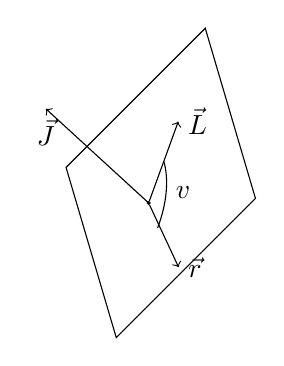
\begin{tikzpicture}[rotate around z=45, rotate around x=-45]
\draw (0,-0.3,0) -- (2.5,-0.3,0) -- (2.5,2.5,0) -- (0,2.5,0) -- cycle;
\draw[->] (1.,1.,0)node[draw,circle,inner sep=0] (o) {} -- (1.5,1.5,2)node[below] {$\vec{J}$};
\draw[->] (o) -- ++(295:0.9cm)node[right] {$\vec{r}$};
\draw[->] (o) -- ++(70:1.1cm)node[right] {$\vec{L}$}node [midway] (aux){};
\draw (aux) arc (0:-50:1) node[midway,right] {$v$};
\end{tikzpicture}

\label{fig:Lenztikz}

\end{figure}

\end{filecontents}


\begin{filecontents}{reducedproblem.tex}

%reduced problem

\begin{tikzpicture}

\node[circle,fill,inner sep=1pt,label=above:M] (M) at (0,0) {}; 
\draw (M)--++(30:1cm) node[circle,fill,inner sep=1pt,label=below:O] (O) {};
\draw[->] (O)--++(30:1.5cm) node[circle,fill,inner sep=1pt,label=above:m,yshift=1pt,xshift=1pt] (m) {} node[midway,above] {$\vec{r}$} ;

\node[circle,fill,inner sep=1pt,below=1cm of O,label=below:O] (O1) {}; 
\draw[->] (O1)--++(30:1.5cm) node[circle,fill,inner sep=1pt,label=above:m,yshift=1pt,xshift=1pt] (m1) {} node[midway,below] {$\vec{r_1}$} ;
\draw[->] (O1)--++(-150:1cm) node[circle,fill,inner sep=1pt,label=above:m,yshift=1pt,xshift=1pt] (m1) {} node[midway,below] {$\vec{r_2}$} ;
%\node (dida) at (7,0) {\parbox{8cm}{Siano m e M due masse puntiformi o a simmetria sferica: O \'e il centro di massa e $\vec{r}=\vec{r_1}-\vec{r_2}$ la distanza relativa.}};

\end{tikzpicture}

\end{filecontents}

\begin{filecontents}{ellipse.tex}

%ellisse

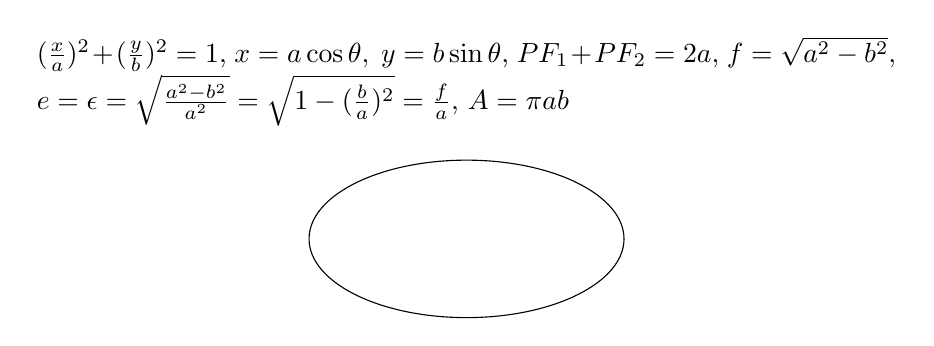
\begin{tikzpicture}

\draw ellipse (2cm and 1cm) node (o) {};
\node (prop) at (0,2) {\parbox{0.9\textwidth}{
$(\frac{x}{a})^2+(\frac{y}{b})^2=1$,
$x=a\cos{\theta},\ y=b\sin{\theta}$,
$PF_1+PF_2=2a$,
$f=\sqrt{a^2-b^2}$,
$e=\epsilon=\sqrt{\frac{a^2-b^2}{a^2}}=\sqrt{1-(\frac{b}{a})^2}=\frac{f}{a}$,
$A=\pi ab$}
};

\end{tikzpicture}

\end{filecontents}%%contain tikz files as filecontents

\addtobeamertemplate{block begin}{\setlength\abovedisplayskip{2pt}\setlength\belowdisplayskip{2pt}\setlength\abovedisplayshortskip{2pt}\setlength\belowdisplayshortskip{2pt}}

\addtobeamertemplate{block begin}{\vspace*{-3pt}}{}
\addtobeamertemplate{block end}{}{\vspace*{-3pt}}

\begin{frame}
  \titlepage
\end{frame}

% Section and subsections will appear in the presentation overview
% and table of contents.
%\frame{\tableofcontents[onlyparts]}

\begin{frame}[label={argomenti}]{Sistemi planetari: Sistema solare}

\tableofcontents[onlyparts]


\end{frame}

\begin{wordonframe}{Perch\'e studio queste cose?? Sviluppi; futuro.}


\end{wordonframe}

\part{Modello planetario}\label{part:planetmodel}
\frame{\partpage}

\part{Fenomenologia sistema solare: pianeti terrestri, giganti gassosi, giganti ghiacciati, sistemi di anelli satelliti e corpi minori}\label{part:solsysphenomen}
\frame{\partpage}

\begin{frame}{this part toc}

\begin{itemize}

\item Pianeti terrestri

\item Giganti gassosi: Giove e Saturno

\item Giganti ghiacciati: Urano, Nettuno

\item Asteroidi: NEO, MB, TNO. Comete

\end{itemize}

\end{frame}

\begin{wordonframe}{Pianeta}

\begin{itemize}
\item Orbita attorno a stella
\item Forma definita equilibrio idrostatico
\item Nella sua orbita non sono presenti distribuzioni di massa comparabili
\end{itemize}

\end{wordonframe}


\section{}

\begin{frame}{Giove}


\end{frame}

\begin{wordonframe}{giove}


\end{wordonframe}

\section{Giove, satelliti e anelli}

\begin{frame}{Giove}


\end{frame}

\begin{wordonframe}{giove}


\end{wordonframe}


\section{Giove, satelliti e anelli}

\begin{frame}{Giove}


\end{frame}

\begin{wordonframe}{giove}


\end{wordonframe}



\part{Evoluzione del sistema solare: forze gravitazionali e non, collisioni.}\label{part:analytic}
\frame{\partpage}

\begin{frame}{this part toc}

\begin{itemize}

\item Evoluzione dinamica del sistema solare

\item Evoluzione collisionale

\end{itemize}


\end{frame}

\section{Giove, satelliti e anelli}

\begin{frame}{Giove}


\end{frame}

\begin{wordonframe}{giove}


\end{wordonframe}

\input{collisions}


\end{document}